\section{Register description}
\regover{
{\hyperref[mjdec-jdec-control-1]{jdec\_control\_1}}&
\\
\hline
{\hyperref[mjdec-jdec-yy-frame-addr]{jdec\_yy\_frame\_addr}}&
\\
\hline
{\hyperref[mjdec-jdec-uv-frame-addr]{jdec\_uv\_frame\_addr}}&
\\
\hline
{\hyperref[mjdec-jdec-control-3]{jdec\_control\_3}}&
\\
\hline
{\hyperref[mjdec-jdec-int-clr]{jdec\_int\_clr}}&
\\
\hline
{\hyperref[mjdec-jdec-fram-push]{jdec\_fram\_push}}&
\\
\hline
{\hyperref[mjdec-jdec-fram-sts]{jdec\_fram\_sts}}&
\\
\hline
{\hyperref[mjdec-jdec-frame-size]{jdec\_frame\_size}}&
\\
\hline
{\hyperref[mjdec-jdec-header-skip]{jdec\_header\_skip}}&
\\
\hline
{\hyperref[mjdec-jp-addr0]{jp\_addr0}}&
\\
\hline
{\hyperref[mjdec-jp-addr1]{jp\_addr1}}&
\\
\hline
{\hyperref[mjdec-jp-addr2]{jp\_addr2}}&
\\
\hline
{\hyperref[mjdec-jp-addr3]{jp\_addr3}}&
\\
\hline
{\hyperref[mjdec-jp-addr4]{jp\_addr4}}&
\\
\hline
{\hyperref[mjdec-jp-addr5]{jp\_addr5}}&
\\
\hline
{\hyperref[mjdec-jp-addr6]{jp\_addr6}}&
\\
\hline
{\hyperref[mjdec-jp-addr7]{jp\_addr7}}&
\\
\hline
{\hyperref[mjdec-jp-addr-8]{jp\_addr\_8}}&
\\
\hline
{\hyperref[mjdec-jp-addr-9]{jp\_addr\_9}}&
\\
\hline
{\hyperref[mjdec-jp-addr-a]{jp\_addr\_a}}&
\\
\hline
{\hyperref[mjdec-jp-addr-b]{jp\_addr\_b}}&
\\
\hline
{\hyperref[mjdec-jp-addr-c]{jp\_addr\_c}}&
\\
\hline
{\hyperref[mjdec-jp-addr-d]{jp\_addr\_d}}&
\\
\hline
{\hyperref[mjdec-jp-addr-e]{jp\_addr\_e}}&
\\
\hline
{\hyperref[mjdec-jp-addr-f]{jp\_addr\_f}}&
\\
\hline
{\hyperref[mjdec-mjdec-debug]{mjdec\_debug}}&
\\
\hline
{\hyperref[mjdec-mjdec-dummy-reg]{mjdec\_dummy\_reg}}&
\\
\hline
}

\subsection{jdec\_control\_1}
\label{mjdec-jdec-control-1}
Address:0x30023000
 \begin{figure}[H]
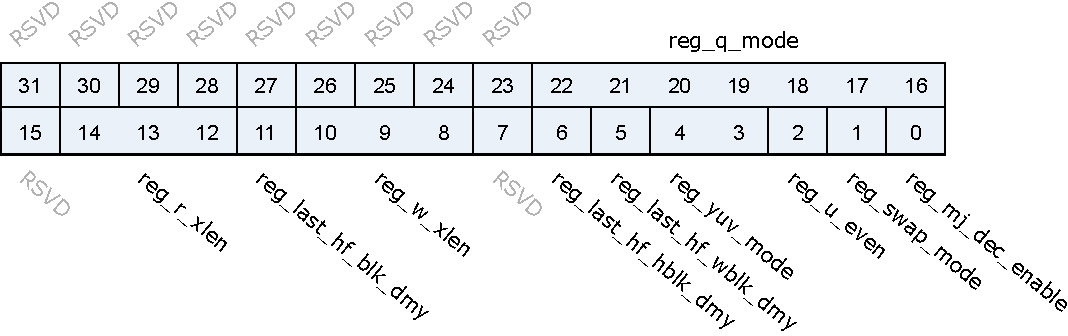
\includegraphics{mjdec_jdec_control_1.pdf}
\end{figure}

\regdes{31:23&RSVD& & & \\\hline
22:16&reg\_q\_mode&r/w&7'd50&Quantization Selection \par 1-75 : Q table selection \par Others : Q100(Lossless)
\\\hline
15&RSVD& & & \\\hline
14:12&reg\_r\_xlen&r/w&3'd3&AXI read burst length setting  \par 3'd0-Single / 3'd1-INCR4 / 3'd2-INCR8 \par 3'd3 - INCR16 / Others - RSVD
\\\hline
11&reg\_last\_hf\_blk\_dmy&r/w&1'b0&JDEC last half block with dummy data 8'h80\\\hline
10:8&reg\_w\_xlen&r/w&3'd3&AXI write burst length setting  \par 3'd0-Single / 3'd1-INCR4 / 3'd2-INCR8 \par 3'd3 - INCR16 / Others - RSVD
\\\hline
7&RSVD& & & \\\hline
6&reg\_last\_hf\_hblk\_dmy&r/w&1'b0&JDEC last half vertical block drop\\\hline
5&reg\_last\_hf\_wblk\_dmy&r/w&1'b0&JDEC last half horizational block drop\\\hline
4:3&reg\_yuv\_mode&r/w&2'd0&YUV format setting \par 2'd0 : YUV420 Planar \par 2'd1 : YUV400 grey scale \par 2'd2 : YUV422 Planar
\\\hline
2&reg\_u\_even&r/w&1'b1&1'b0 - U is odd byte of UV frame / V is even byte of UV frame \par 1'b1 - U is even byte of UV frame / V is odd byte of UV frame
\\\hline
1&reg\_swap\_mode&r/w&1'b0&JDEC YUV Memory swap mode\\\hline
0&reg\_mj\_dec\_enable&r/w&1'b0&JDEC Enable\\\hline

}
\subsection{jdec\_yy\_frame\_addr}
\label{mjdec-jdec-yy-frame-addr}
Address:0x30023008
 \begin{figure}[H]
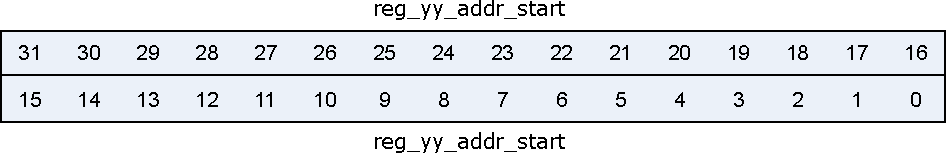
\includegraphics{mjdec_jdec_yy_frame_addr.pdf}
\end{figure}

\regdes{31:0&reg\_yy\_addr\_start&r/w&32'h80000000&Memory start address of Y frame\\\hline

}
\subsection{jdec\_uv\_frame\_addr}
\label{mjdec-jdec-uv-frame-addr}
Address:0x3002300c
 \begin{figure}[H]
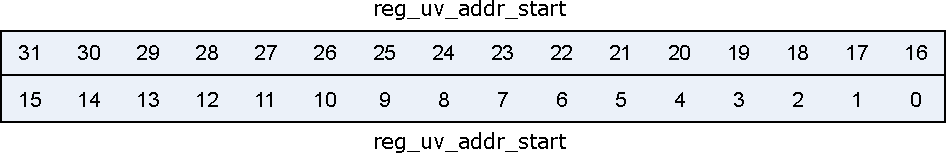
\includegraphics{mjdec_jdec_uv_frame_addr.pdf}
\end{figure}

\regdes{31:0&reg\_uv\_addr\_start&r/w&32'h80000000&Memory start address of UV frame\\\hline

}
\subsection{jdec\_control\_3}
\label{mjdec-jdec-control-3}
Address:0x3002301c
 \begin{figure}[H]
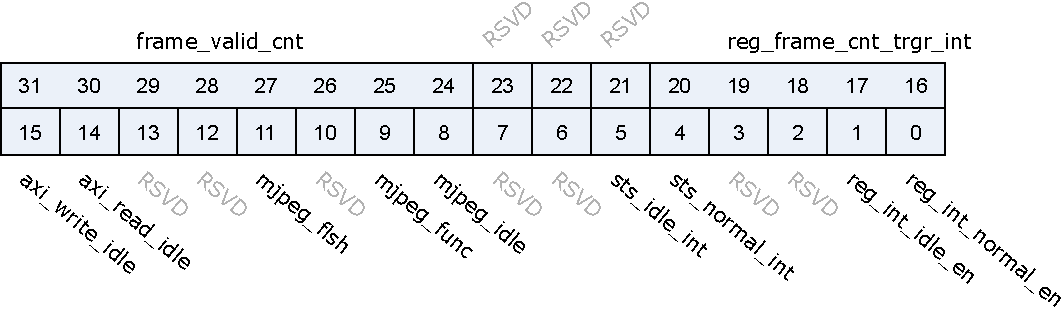
\includegraphics{mjdec_jdec_control_3.pdf}
\end{figure}

\regdes{31:24&frame\_valid\_cnt&r&8'd0&Frame count valid in status\\\hline
23:21&RSVD& & & \\\hline
20:16&reg\_frame\_cnt\_trgr\_int&r/w&5'd0&Frame threshold to issue interrupt\\\hline
15&axi\_write\_idle&r&1'b0&AXI write bus idle state\\\hline
14&axi\_read\_idle&r&1'b0&AXI read bus idle state\\\hline
13:12&RSVD& & & \\\hline
11&mjpeg\_flsh&r&1'b0&MJPEG in flush state\\\hline
10&RSVD& & & \\\hline
9&mjpeg\_func&r&1'b0&MJPEG in HW function state\\\hline
8&mjpeg\_idle&r&1'b1&MJPEG in idle state\\\hline
7:6&RSVD& & & \\\hline
5&sts\_idle\_int&r&1'b0&Normal Write interrupt status\\\hline
4&sts\_normal\_int&r&1'b0&Normal Write interrupt status\\\hline
3:2&RSVD& & & \\\hline
1&reg\_int\_idle\_en&r/w&1'b0&Back idle interrupt enable\\\hline
0&reg\_int\_normal\_en&r/w&1'b1&Normal Write interrupt enable\\\hline

}
\subsection{jdec\_int\_clr}
\label{mjdec-jdec-int-clr}
Address:0x30023020
 \begin{figure}[H]
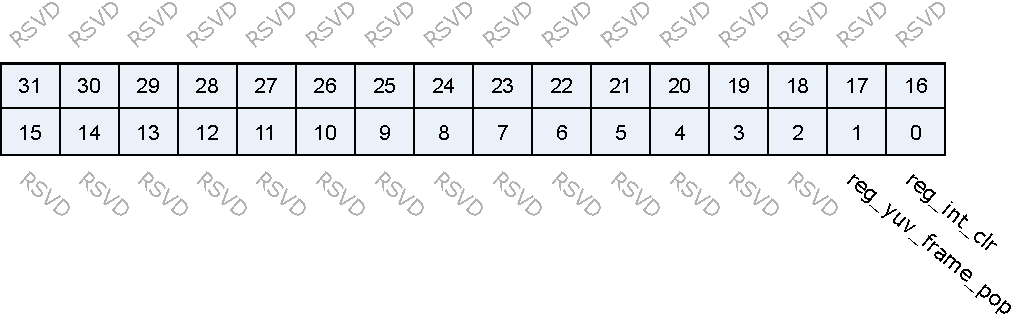
\includegraphics{mjdec_jdec_int_clr.pdf}
\end{figure}

\regdes{31:2&RSVD& & & \\\hline
1&reg\_yuv\_frame\_pop&w1p&1'b0&Wrire this bit with 1'b1 to pop yuv frame cnt\\\hline
0&reg\_int\_clr&w1p&1'b0&Wrire this bit with 1'b1 to trigger interrupt clear\\\hline

}
\subsection{jdec\_fram\_push}
\label{mjdec-jdec-fram-push}
Address:0x30023024
 \begin{figure}[H]
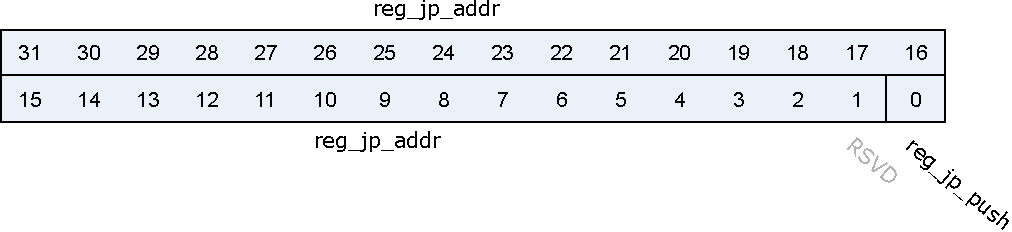
\includegraphics{mjdec_jdec_fram_push.pdf}
\end{figure}

\regdes{31:2&reg\_jp\_addr&r/w&30'h0&JPEG Start Addr\\\hline
1&RSVD& & & \\\hline
0&reg\_jp\_push&w1p&1'b0&Wrire this bit with 1'b1 to push jpg frame\\\hline

}
\subsection{jdec\_fram\_sts}
\label{mjdec-jdec-fram-sts}
Address:0x30023028
 \begin{figure}[H]
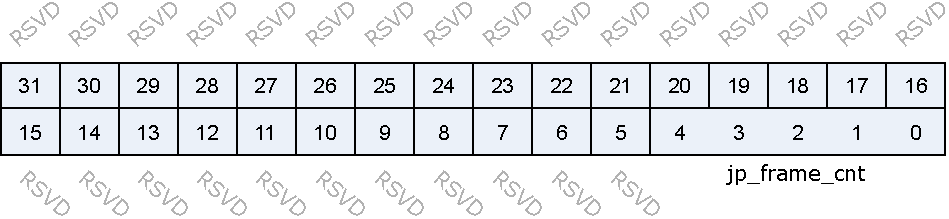
\includegraphics{mjdec_jdec_fram_sts.pdf}
\end{figure}

\regdes{31:5&RSVD& & & \\\hline
4:0&jp\_frame\_cnt&r&5'h0&JPEG FIFO frame cnt\\\hline

}
\subsection{jdec\_frame\_size}
\label{mjdec-jdec-frame-size}
Address:0x3002302c
 \begin{figure}[H]
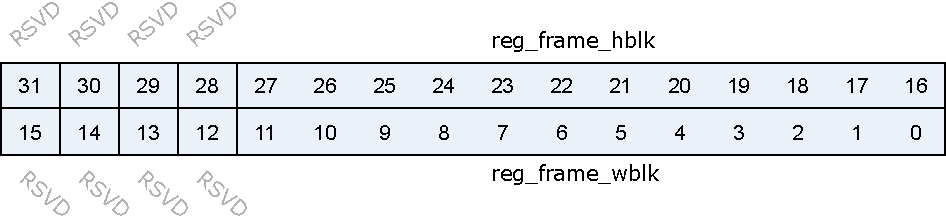
\includegraphics{mjdec_jdec_frame_size.pdf}
\end{figure}

\regdes{31:28&RSVD& & & \\\hline
27:16&reg\_frame\_hblk&r/w&8'd20&Frame total vertical block count\\\hline
15:12&RSVD& & & \\\hline
11:0&reg\_frame\_wblk&r/w&8'd15&Frame total horizational block count\\\hline

}
\subsection{jdec\_header\_skip}
\label{mjdec-jdec-header-skip}
Address:0x30023030
 \begin{figure}[H]
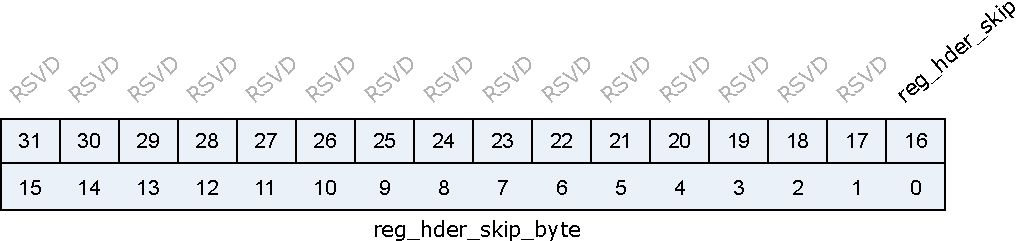
\includegraphics{mjdec_jdec_header_skip.pdf}
\end{figure}

\regdes{31:17&RSVD& & & \\\hline
16&reg\_hder\_skip&r/w&1'b0&Skip JPEG stream header enable\\\hline
15:0&reg\_hder\_skip\_byte&r/w&16'd0&Skip JPEG stream header byte\\\hline

}
\subsection{jp\_addr0}
\label{mjdec-jp-addr0}
Address:0x30023040
 \begin{figure}[H]
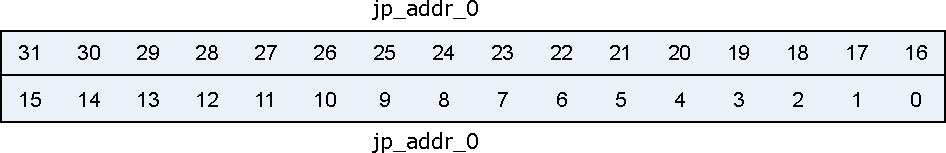
\includegraphics{mjdec_jp_addr0.pdf}
\end{figure}

\regdes{31:0&jp\_addr\_0&r&32'd0&JPEG PIC 0 Start address\\\hline

}
\subsection{jp\_addr1}
\label{mjdec-jp-addr1}
Address:0x30023044
 \begin{figure}[H]
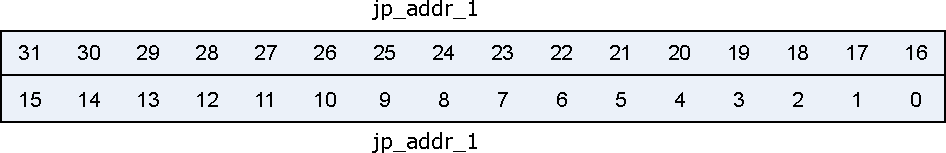
\includegraphics{mjdec_jp_addr1.pdf}
\end{figure}

\regdes{31:0&jp\_addr\_1&r&32'd0&JPEG PIC 1 Start address\\\hline

}
\subsection{jp\_addr2}
\label{mjdec-jp-addr2}
Address:0x30023048
 \begin{figure}[H]
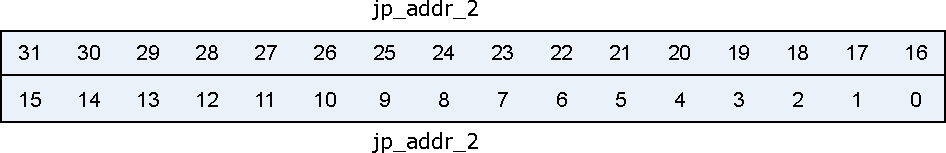
\includegraphics{mjdec_jp_addr2.pdf}
\end{figure}

\regdes{31:0&jp\_addr\_2&r&32'd0&JPEG PIC 2 Start address\\\hline

}
\subsection{jp\_addr3}
\label{mjdec-jp-addr3}
Address:0x3002304c
 \begin{figure}[H]
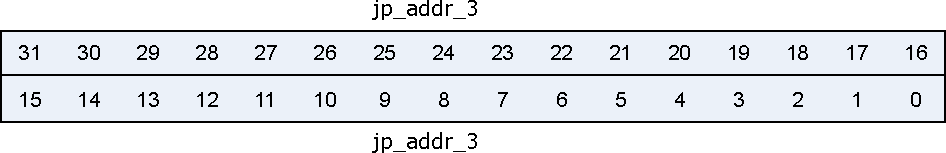
\includegraphics{mjdec_jp_addr3.pdf}
\end{figure}

\regdes{31:0&jp\_addr\_3&r&32'd0&JPEG PIC 3 Start address\\\hline

}
\subsection{jp\_addr4}
\label{mjdec-jp-addr4}
Address:0x30023050
 \begin{figure}[H]
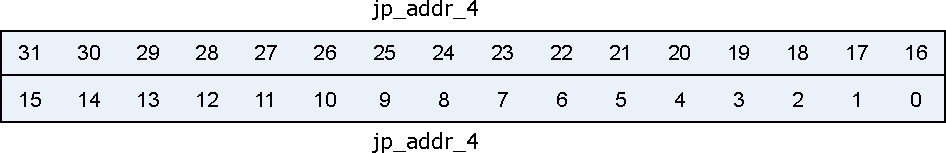
\includegraphics{mjdec_jp_addr4.pdf}
\end{figure}

\regdes{31:0&jp\_addr\_4&r&32'd0&JPEG PIC 4 Start address\\\hline

}
\subsection{jp\_addr5}
\label{mjdec-jp-addr5}
Address:0x30023054
 \begin{figure}[H]
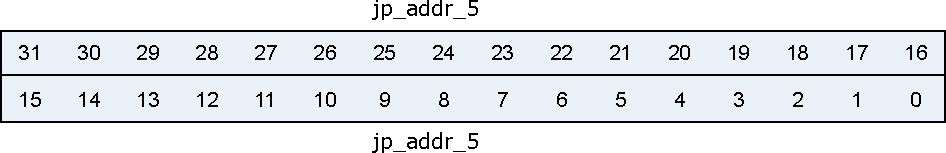
\includegraphics{mjdec_jp_addr5.pdf}
\end{figure}

\regdes{31:0&jp\_addr\_5&r&32'd0&JPEG PIC 5 Start address\\\hline

}
\subsection{jp\_addr6}
\label{mjdec-jp-addr6}
Address:0x30023058
 \begin{figure}[H]
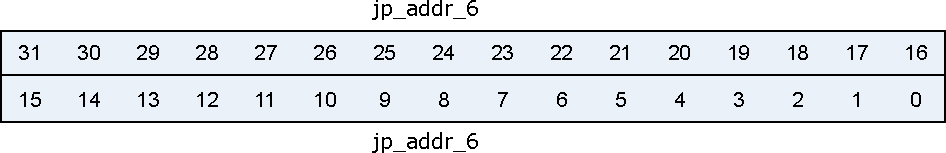
\includegraphics{mjdec_jp_addr6.pdf}
\end{figure}

\regdes{31:0&jp\_addr\_6&r&32'd0&JPEG PIC 6 Start address\\\hline

}
\subsection{jp\_addr7}
\label{mjdec-jp-addr7}
Address:0x3002305c
 \begin{figure}[H]
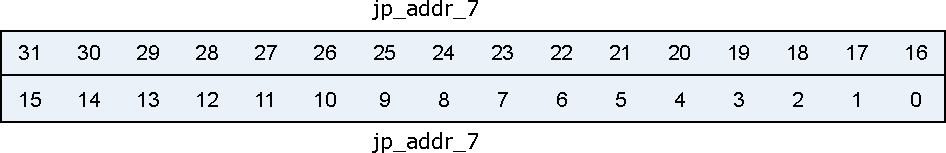
\includegraphics{mjdec_jp_addr7.pdf}
\end{figure}

\regdes{31:0&jp\_addr\_7&r&32'd0&JPEG PIC 7 Start address\\\hline

}
\subsection{jp\_addr\_8}
\label{mjdec-jp-addr-8}
Address:0x30023060
 \begin{figure}[H]
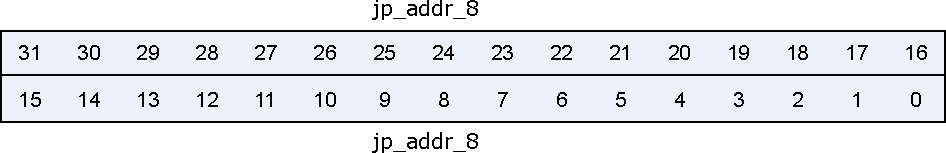
\includegraphics{mjdec_jp_addr_8.pdf}
\end{figure}

\regdes{31:0&jp\_addr\_8&r&32'd0&JPEG PIC 8 Start address\\\hline

}
\subsection{jp\_addr\_9}
\label{mjdec-jp-addr-9}
Address:0x30023064
 \begin{figure}[H]
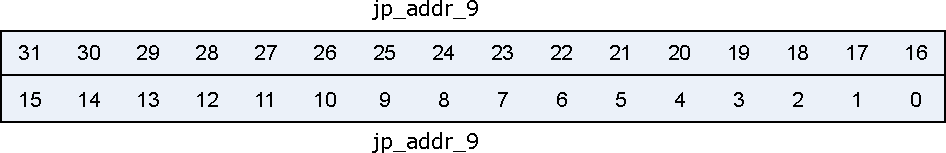
\includegraphics{mjdec_jp_addr_9.pdf}
\end{figure}

\regdes{31:0&jp\_addr\_9&r&32'd0&JPEG PIC 9 Start address\\\hline

}
\subsection{jp\_addr\_a}
\label{mjdec-jp-addr-a}
Address:0x30023068
 \begin{figure}[H]
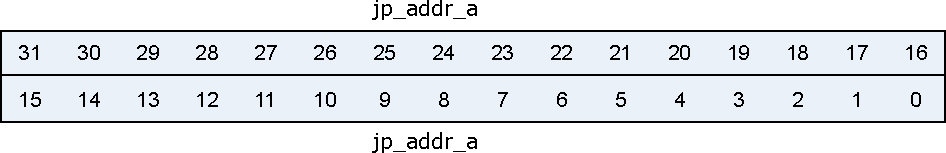
\includegraphics{mjdec_jp_addr_a.pdf}
\end{figure}

\regdes{31:0&jp\_addr\_a&r&32'd0&JPEG PIC A Start address\\\hline

}
\subsection{jp\_addr\_b}
\label{mjdec-jp-addr-b}
Address:0x3002306c
 \begin{figure}[H]
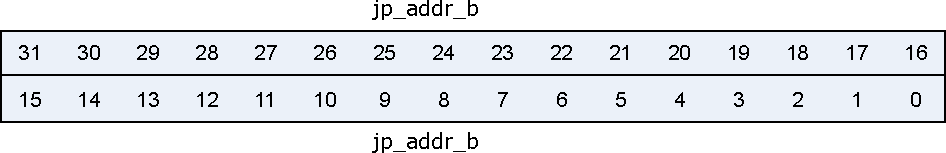
\includegraphics{mjdec_jp_addr_b.pdf}
\end{figure}

\regdes{31:0&jp\_addr\_b&r&32'd0&JPEG PIC B Start address\\\hline

}
\subsection{jp\_addr\_c}
\label{mjdec-jp-addr-c}
Address:0x30023070
 \begin{figure}[H]
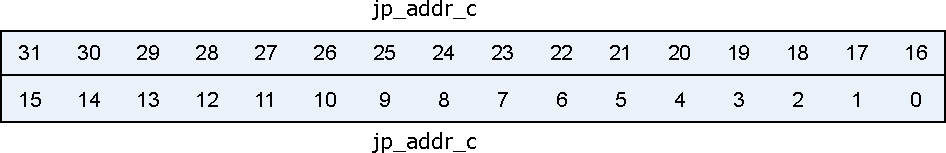
\includegraphics{mjdec_jp_addr_c.pdf}
\end{figure}

\regdes{31:0&jp\_addr\_c&r&32'd0&JPEG PIC C Start address\\\hline

}
\subsection{jp\_addr\_d}
\label{mjdec-jp-addr-d}
Address:0x30023074
 \begin{figure}[H]
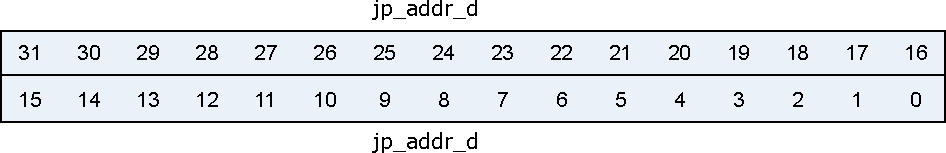
\includegraphics{mjdec_jp_addr_d.pdf}
\end{figure}

\regdes{31:0&jp\_addr\_d&r&32'd0&JPEG PIC D Start address\\\hline

}
\subsection{jp\_addr\_e}
\label{mjdec-jp-addr-e}
Address:0x30023078
 \begin{figure}[H]
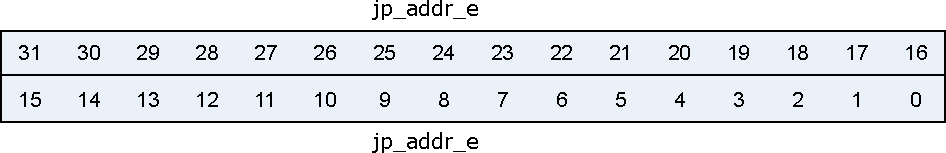
\includegraphics{mjdec_jp_addr_e.pdf}
\end{figure}

\regdes{31:0&jp\_addr\_e&r&32'd0&JPEG PIC E Start address\\\hline

}
\subsection{jp\_addr\_f}
\label{mjdec-jp-addr-f}
Address:0x3002307c
 \begin{figure}[H]
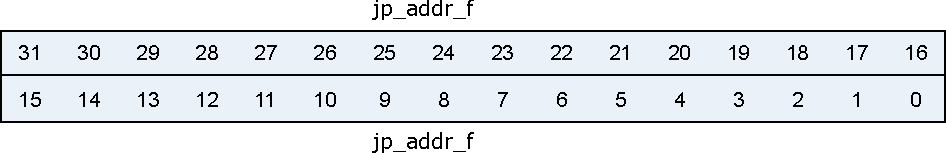
\includegraphics{mjdec_jp_addr_f.pdf}
\end{figure}

\regdes{31:0&jp\_addr\_f&r&32'd0&JPEG PIC F Start address\\\hline

}
\subsection{mjdec\_debug}
\label{mjdec-mjdec-debug}
Address:0x300231f0
 \begin{figure}[H]
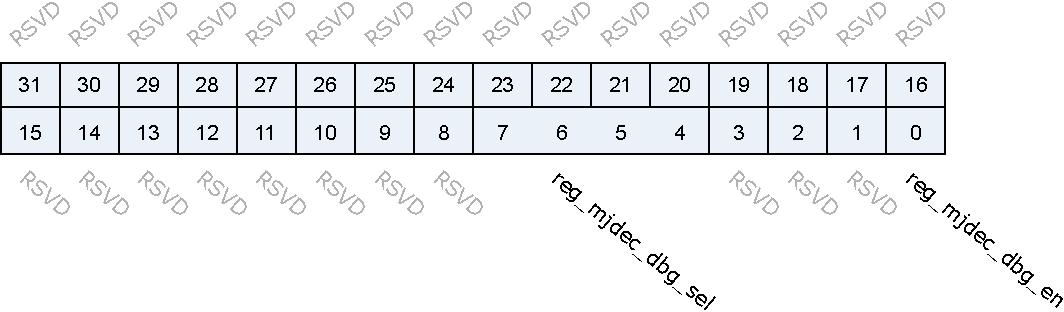
\includegraphics{mjdec_mjdec_debug.pdf}
\end{figure}

\regdes{31:8&RSVD& & & \\\hline
7:4&reg\_mjdec\_dbg\_sel&r/w&4'd0&MJPEG debgu flag selection\\\hline
3:1&RSVD& & & \\\hline
0&reg\_mjdec\_dbg\_en&r/w&1'b0&MJPEG debgu flag enable\\\hline

}
\subsection{mjdec\_dummy\_reg}
\label{mjdec-mjdec-dummy-reg}
Address:0x300231fc
 \begin{figure}[H]
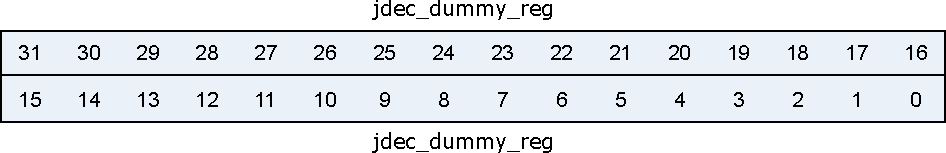
\includegraphics{mjdec_mjdec_dummy_reg.pdf}
\end{figure}

\regdes{31:0&jdec\_dummy\_reg&r/w&32'd0&Dummy R/W register\\\hline

}
